\section{Baseline}

首先我制作了 \texttt{baselineSearch} 函数, 其在测试集 8000 上的效率是约每秒 100 次搜索.

\begin{figure}[H]
    \centering
    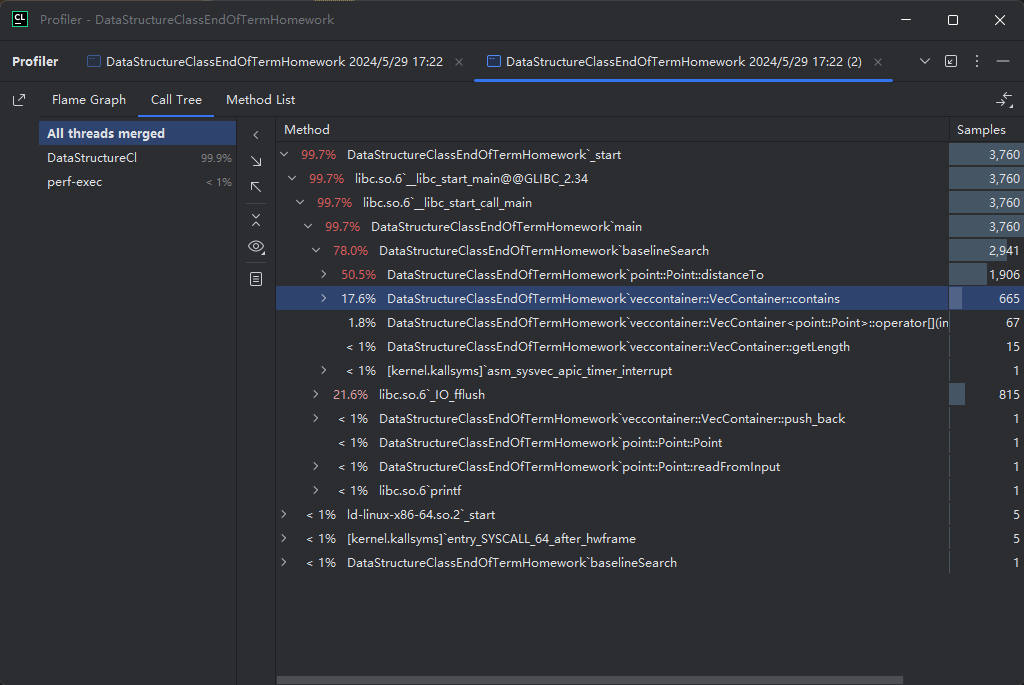
\includegraphics[width=0.5\textwidth]{img/baseline-profile}
    \caption{Baseline Profile}
\end{figure}

发现选中项 \texttt{contains} 有不必要的时间占用.


\section{Baseline With HashSet}

于是我将 \texttt{HashSet} 应用到 \texttt{baselineSearch} 索引的保存中, 并将 \texttt{hashSet} 设置为 1000.

\begin{figure}[H]
    \centering
    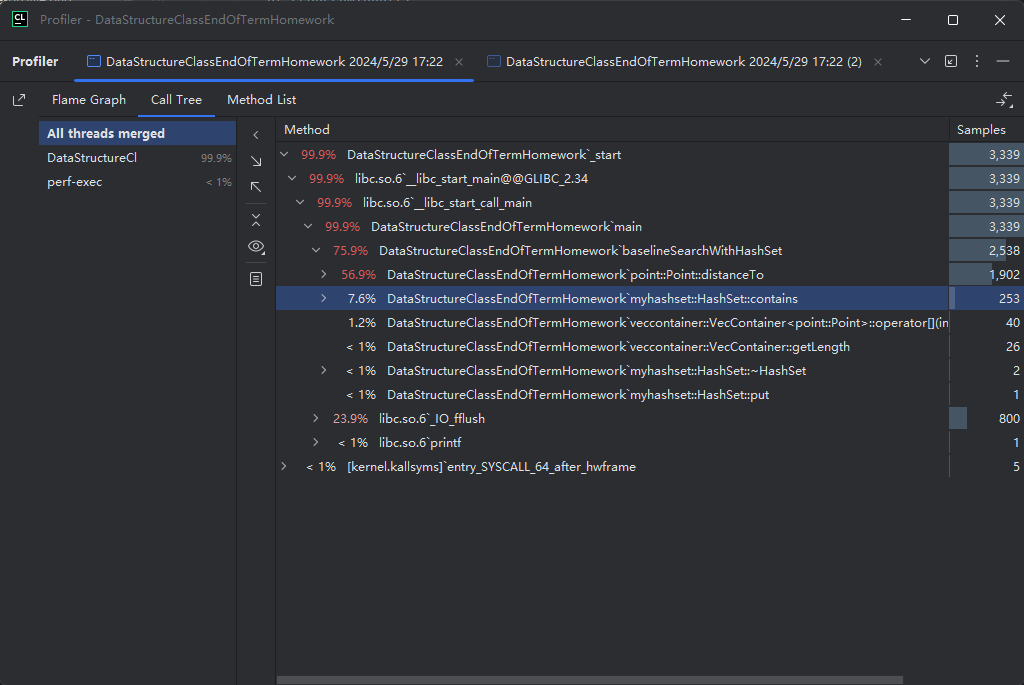
\includegraphics[width=0.5\textwidth]{img/baseline-with-hashset-profile}
    \caption{Baseline with HashSet Profile}
\end{figure}

得到了小许优化.

\subsection{结果}

\begin{figure}[H]
    \centering
    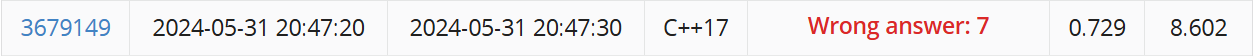
\includegraphics[width=0.8\textwidth]{img/baseline-score}
    \caption{Baseline Score}
\end{figure}

惨不忍睹.


\section{HNSW}

通过\href{https://www.bilibili.com/video/BV14u4y1A7fB?p=4}{向量数据库}视频, 我了解到了 HNSW 算法,
用于查找与目标向量最接近的向量.

其大致的思路是:

\begin{enumerate}
    \item 创建多个层, 不同的层从稀疏到密集.
    \item 算法分为两个步骤, 我称之为 Build 和 Search:
    \begin{enumerate}
        \item Build: 创建不同层次的图, 以不同的频率添加向量到不同的层之中, 添加向量时让其和原先在图中和其最靠近的 N\_LINK 个向量建立连接.
        \item Search:
        \begin{enumerate}
            \item 先在最稀疏的层中选一个节点开始进行贪婪地查找最接近的向量, 直到图中节点没有邻居比其更加靠近目标向量, 得到局部最小值节点.
            \item 从上一层的局部最小值节点开始, 在更加密集的下一层中, 重复上述步骤, 直到最底层, 得到近似的和目标向量最接近的节点.
        \end{enumerate}
    \end{enumerate}
\end{enumerate}

\begin{figure}[H]
    \centering
    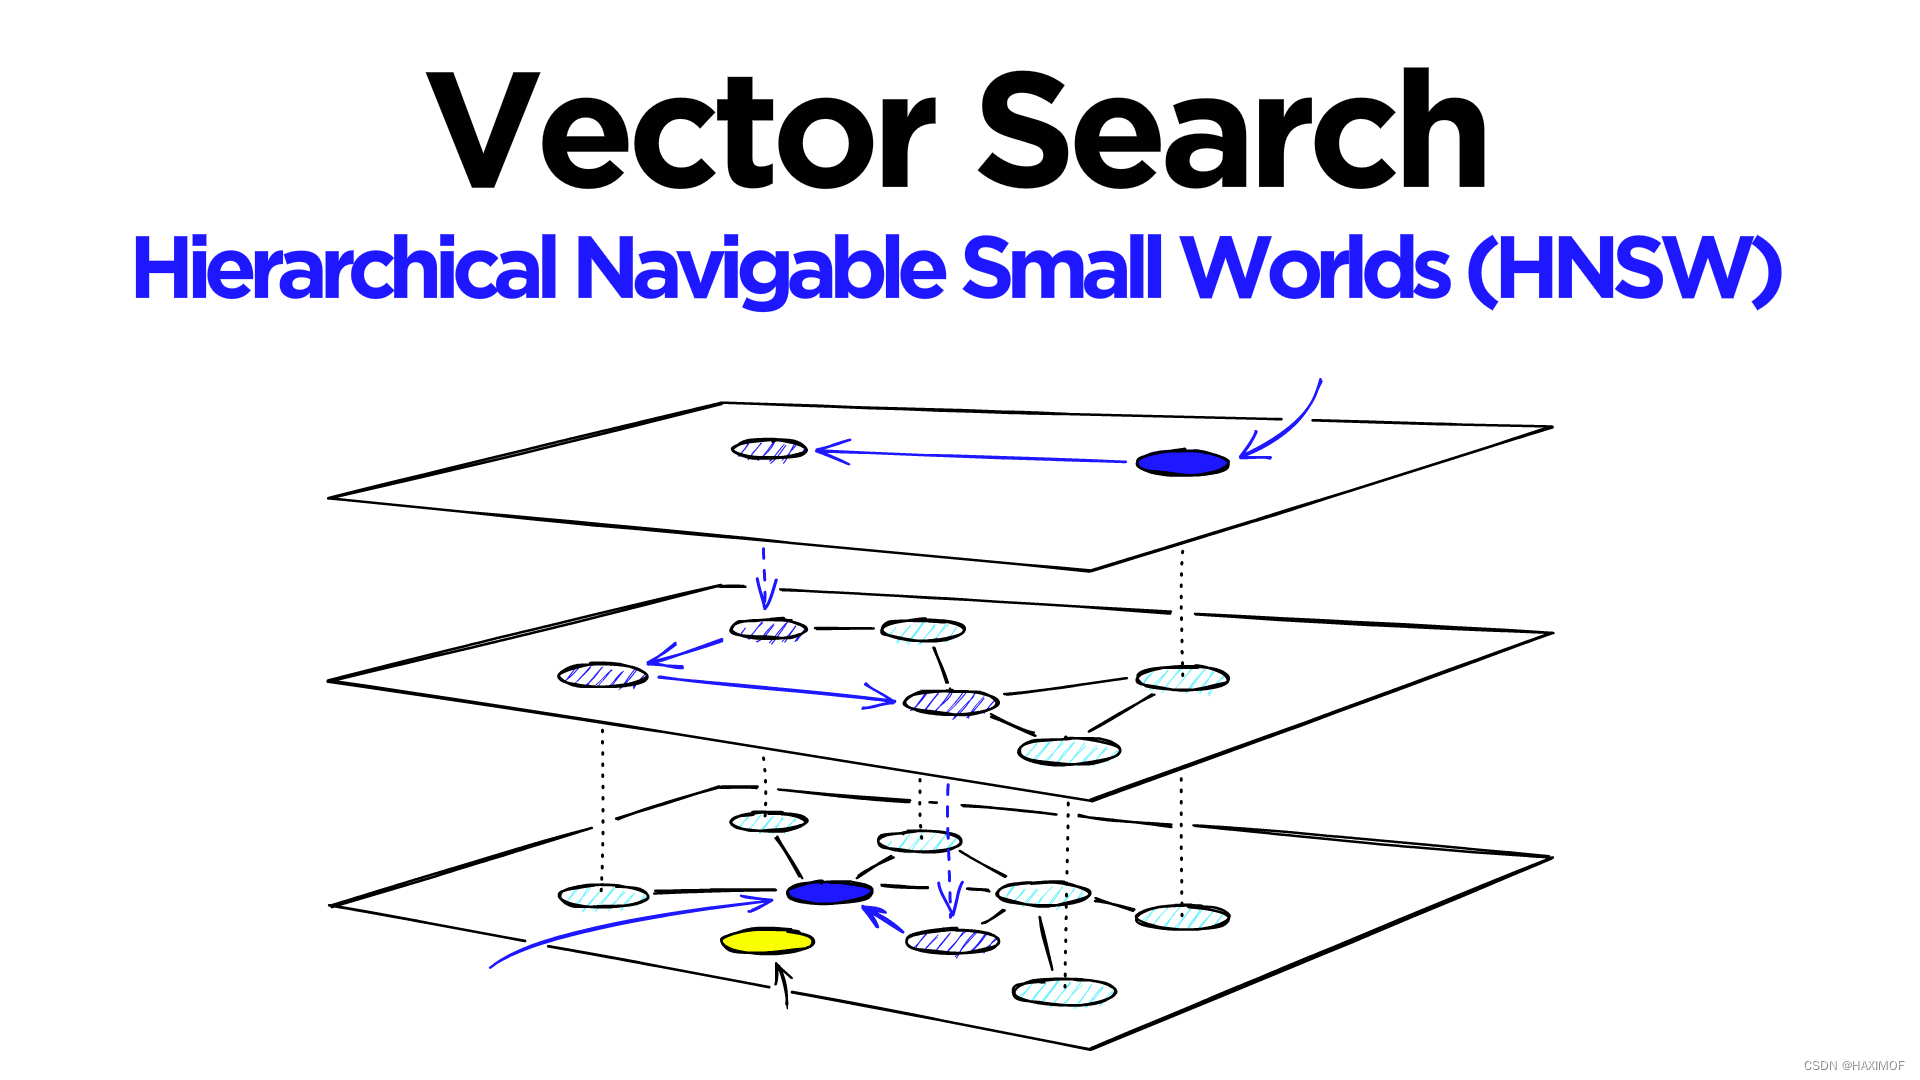
\includegraphics[width=0.8\textwidth]{hnsw-intro-img}
    \caption{HNSW Introduction}
\end{figure}

在我的理解中, 此算法在 Build 中也需要使用 Search 中的部分步骤, 其中最困扰我的是如何进行 KNN 搜索.

\subsection{HNSW-KNN}

但是我第一眼看去 HNSW 只能用于查找最近的一个向量, 并没有直接看出如何使用 HNSW 应用于 KNN 问题上.

\subsubsection{优先级队列}

于是我问 GPT, 它说用优先级队列来实现最近 k 个节点的获取, 但是它给出的具体解决方案近乎胡扯,
于是我只能自己想具体实现.

在我最初的设想中: 优先级队列中队列首位元素是距离目标点最远的点, 探索时每次循环弹出队列首位元素,
然后如果弹出的节点有比此节点距离目标向量更近的邻居节点, 且此邻居节点不在优先级队列内,
则将邻居节点添加进优先级队列中.
总结就是: 弹出最远的, 放入更近的.

\subsubsection{优先级队列特殊情况}

如果探索完, 结果没有 k 个节点, 可能的情况为:

\begin{enumerate}
    \item 层中没有足够的点.
    \item 搜索的起始点和目标点足够近.
\end{enumerate}

\subsubsection{优先级队列特殊情况的解决思路}

对于第一点, 我的解决思路是直接返回层中的所有节点而不进行搜索.

对于第二点, 我自己想的思路是, 如果优先级队列的元素数量没有达到 k 那就不检查邻居节点与目标向量的距离是否更近,
直接加入队列, 但重复性还是要检查的.\label{repetitive-inspection}

\subsubsection{解决优先级队列比较里的重复计算和重复性检查}

要把优先级队列应用下来, 还需要一个步骤: 缓冲每个节点和目标向量的距离.
原因是在优先级队列中, 需要进行多次比较, 若不缓冲距离则会造成大量的重复的运算.

对此我的设计是:
每个 Layer 维护一个独特的 \texttt{searchBatch:int}, 用于记录搜索批次, 每当搜索的目标节点或使用的优先级队列发生变化,
此值自增.
Layer 中的每个 GraphNode 添加三个字段: \texttt{{batch:int, inQueue:bool, distance:double}},
分别代表缓冲的距离所属的搜索批次, 是否在队列里和缓冲的距离.

这三个字段不仅可以减少重复的计算, 还能用于\hyperref[repetitive-inspection]{重复性检查},
如果 \texttt{batch != searchBatch}, 就说明此节点在此次搜索中没有被涉及到,
此时 \texttt{inQueue} 和 \texttt{distance} 的值需要重新设置和计算.
如果 \texttt{batch == searchBatch}, 说明此次搜索层涉及过此节点, 那么 \texttt{distance} 字段可以直接使用, \texttt{inQueue}
字段用来判断此节点是否在优先级队列里, 防止反复添加.

最后放进优先级队列里的是 GraphNode 的指针, 同时传入一个比较函数给优先级队列, 用于取得 \texttt{distance} 并比较.
此处的设计一开始困扰了我一会, 我的几个原有的想法是:

\begin{enumerate}
    \item 优先级队列里存放 GraphNode 的包裹类, 重载比较运算符.
    \item 优先级队列里存放 GraphNode 在 Layer 中的索引.
\end{enumerate}

这几个想法由于以下缺陷而取消了:

\begin{enumerate}
    \item 包裹类内存开销太大, 每次搜索都要进行多次内存的分配, 且查找值时不方便.
    \item 如果只传入索引, 那么在比较时获取 \texttt{distance} 的值就需要一个 Layer 的引用, 于是在比较函数中就需要拥有 Layer 的指针,
    而获取 Layer 的引用比较困难, 会使代码的耦合性变高.
\end{enumerate}

\subsubsection{自己想的优先级队列搜索步骤}

\textbf{注意}:
以下步骤中,

\begin{enumerate}
    \item 每次使用节点的缓冲距离时, 需要提前计算.
    \item 每次从优先级队列中放入值前需要设置 \texttt{inQueue = true}.
    \item 每次从优先级队列中弹出值时需要设置 \texttt{inQueue = false}.
\end{enumerate}

步骤为:

\begin{enumerate}
    \item 如果 Layer 的节点数量小于等于 k, 直接把 Layer 中所有的节点索引返回.
    \item 从 Layer 中的前 k 个节点开始, 把这些节点放入优先级队列 (pq: \texttt{PriorityQueue<GraphNode *>},
    堆顶存放着距离最远的节点).
    \item 循环, 直到 pq 为空 (pq 为空估计不会出现):
    \begin{enumerate}
        \item 弹出 pq 顶上的元素 \texttt{node}.
        \item 遍历 \texttt{node} 的每个邻居, 当邻居的距离比 \texttt{node} 近时才添加此邻居到 pq 内.
        \item 如果此 \texttt{node} 没有邻居被添加, 结束循环.
    \end{enumerate}
    \item 丢弃 pq 中的多余元素, 直到 pq 剩下 k 个元素.
    \item 将这 k 个元素倒序放在 Vec 中 (distance 字段最小的放在 Vec 0 号位置), 返回.
\end{enumerate}

\subsubsection{错误, 推倒重来}

在编写完上述思路的代码, 准备写层间搜索的衔接时, 我发现以上方法的一个致命的错误:

\begin{figure}[H]
    \centering
    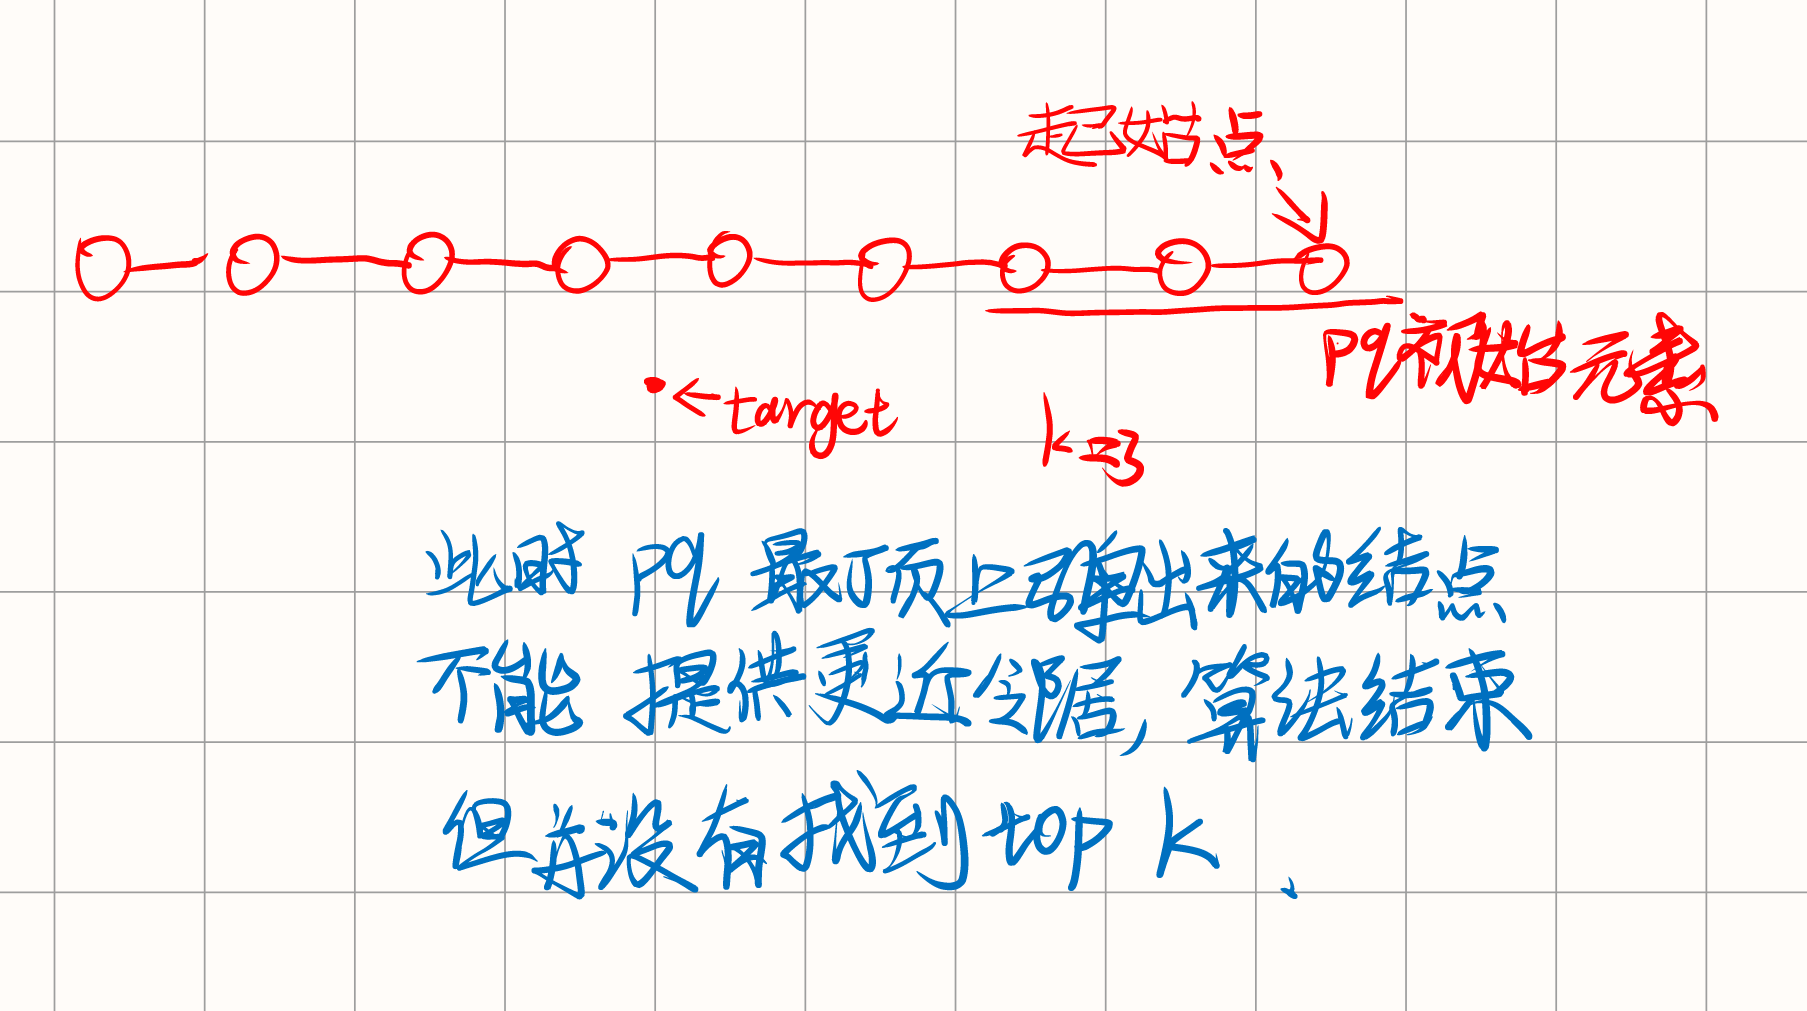
\includegraphics[width=0.8\textwidth]{img/miscase}
    \caption{Miscase}
\end{figure}

\subsection{靠近后拓展}

上述方法失败之后, 我想出了另外一个方法: 先在层内找到距离目标向量最接近的节点, 然后以此节点为起始节点,
拓展 k 个节点, 以此实现 KNN 问题.

拓展的方式是给定一个节点, 从此节点开始以广度优先的方式增添节点, 直到增添到了 k 个节点, 返回这些节点所代表的值.

HNSW 算法实践后, 速度相比 Baseline 有大幅提升, 再把链表的取值用自制迭代器的形式进行优化, 减少冗余的指针游走,
最终在测试集 8000 上的总搜索速度可以到 1 秒左右 (N\_LINK 为 3), 但准确率不尽人意.

速度 (avg 表示每秒进行的搜索次数):

\begin{figure}[H]
    \centering
    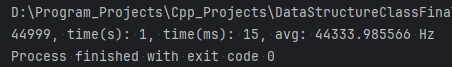
\includegraphics[width=0.8\textwidth]{img/hnsw-topk-efficiency}
    \caption{HNSW Top-K Efficiency}
\end{figure}

准确率样本 (左边是当前方法搜索出来的向量和目标向量的距离, 右边是 Baseline 结果):

\begin{figure}[H]
    \centering
    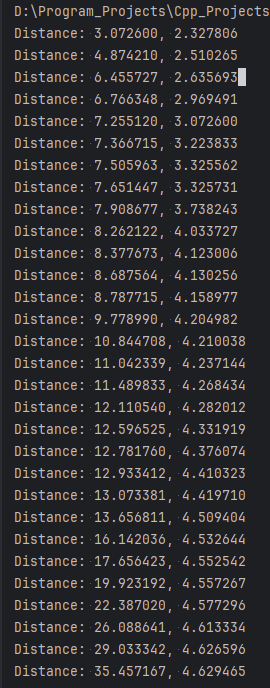
\includegraphics[width=0.3\textwidth]{img/hnsw-topk-accuracy-sample}
    \caption{HNSW Top-K Accuracy Sample}
\end{figure}

由图可知, 此拓展方式产生的 KNN 召回率结果太差, 可以说就是 $0\%$.

\subsection{查阅论文和开源项目}

论文: \href{https://arxiv.org/pdf/1603.09320}{Efficient and robust approximate nearest neighbor search using Hierarchical Navigable Small World graphs}

开源项目: \href{https://github.com/nmslib/hnswlib}{hnswlib}

浏览了论文中对 HNSW 算法的描述后, 我一层一层地分析项目中的代码,
最终找到了此项目中的 \href{../reference/hnswlib/hnswalg.h}{knn 搜索方法: searchBaseLayerST},
把此方法的几个分支简化 (假定 \texttt{bare\_bone\_search} 为 true) 后, 发现方法在搜索时使用了两个优先级队列,
一个优先级队列是正序的, 另一个是倒序的.

这个分支的搜索思路是:

\begin{enumerate}
    \item 同时维护一个结果优先级队列 rq 和一个候选者优先级队列 cq, rq 就是返回值对应的队列.
    \item 把起始节点放入 rq 和 cq.
    \item 循环, 直到 cq 为空:
    \begin{enumerate}
        \item 从 cq 中取出距离目标向量最短的节点 nn.
        \item 如果 nn 比下界还要大 (下界指的是 rq 中距离目标向量最远的节点对应的距离) 则结束循环.
        \item 遍历所有 nn 的没被探索过的邻居 ng:  (被加入到 rq 或者 cq 过则说明被探索过)
        \begin{enumerate}
            \item 如果 ng 的距离比下界小则把 ng 加入 cq 和 rq.
            \item 删除 rq 中的距离最远的几个节点, 直到 rq 尺寸小于等于 k.
        \end{enumerate}
    \end{enumerate}
    \item 取出 rq 的节点作为返回值 (循环中已经保证其尺寸小于等于 k).
\end{enumerate}

此算法相比我自己想的优先级队列搜索, 令我为之震惊的点在于其使用两个优先级队列,
每次循环弹出队列中最近的节点进行探索而不是最远的节点, 还有其使用下界进行判断的方式也令我大开眼界.

我将这个算法和结合 \href{../src/hnsw/Layer.cpp}{searchNearestNode} 使用,形成了 HNSW 算法 KNN 搜索部分.

\subsection{结果}

\begin{figure}[H]
    \centering
    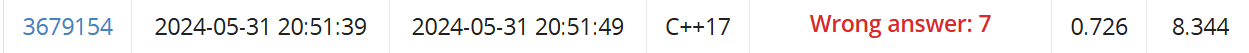
\includegraphics[width=0.8\textwidth]{img/hnsw-knn-score}
    \caption{HNSW KNN Score}
\end{figure}

第一次提交时,此分数让我有点失望,7 分的分数驱使我不断反复创建二维数据集反复测试准确性,在各种测试集上,
其显示的结果大致都如以下输出,召回率十分低:

\begin{verbatim}
            HNSW   Baseline                   HNSW  Baseline
Node:       7399:      6164, 	Distance: 2.969491, 2.327806
Node:        271:      3151, 	Distance: 4.204982, 2.510265
Node:       2427:      7996, 	Distance: 4.331919, 2.635693
Node:       7636:      7399, 	Distance: 4.670664, 2.969491
Node:       7415:      5568, 	Distance: 5.209835, 3.072600
Node:       5968:      7346, 	Distance: 5.450563, 3.223833
Node:       7769:       974, 	Distance: 5.527832, 3.325562
Node:        407:      5588, 	Distance: 5.820290, 3.325731
Node:       2921:       766, 	Distance: 5.860978, 3.738243
Node:       3653:      4222, 	Distance: 5.956301, 4.033727
Node:         56:      6309, 	Distance: 5.979393, 4.123006
Node:       7477:      3586, 	Distance: 6.249059, 4.130256
Node:       6353:      3771, 	Distance: 6.266310, 4.158977
Node:        199:       271, 	Distance: 6.335025, 4.204982
Node:        143:      6780, 	Distance: 6.611314, 4.210038
Node:       5940:      5613, 	Distance: 6.762243, 4.237144
Node:       5657:      4479, 	Distance: 6.766348, 4.268434
Node:       6398:      3673, 	Distance: 6.857042, 4.282012
Node:       5173:      2427, 	Distance: 6.887219, 4.331919
Node:       4997:      4762, 	Distance: 7.156574, 4.376074
Node:       7049:      3239, 	Distance: 7.348852, 4.410323
Node:       3473:      3915, 	Distance: 7.376329, 4.419710
Node:       7749:      2220, 	Distance: 7.424413, 4.509404
Node:       7734:      2714, 	Distance: 7.467890, 4.532644
Node:       1175:      2070, 	Distance: 7.702319, 4.552542
Node:       3026:      1260, 	Distance: 7.765935, 4.557267
Node:       6934:      1736, 	Distance: 7.768849, 4.577296
Node:        146:      1164, 	Distance: 7.918658, 4.613334
Node:       4823:      6265, 	Distance: 8.089707, 4.626596
Node:       7600:      6202, 	Distance: 8.109049, 4.629465
\end{verbatim}

\subsection{陷入局部最小值}

在分析画图过程中,我发现我写的算法里的问题: 容易陷入局部最小值.

下图显示了为何会陷入局部最小值.

\begin{figure}[H]
    \centering
    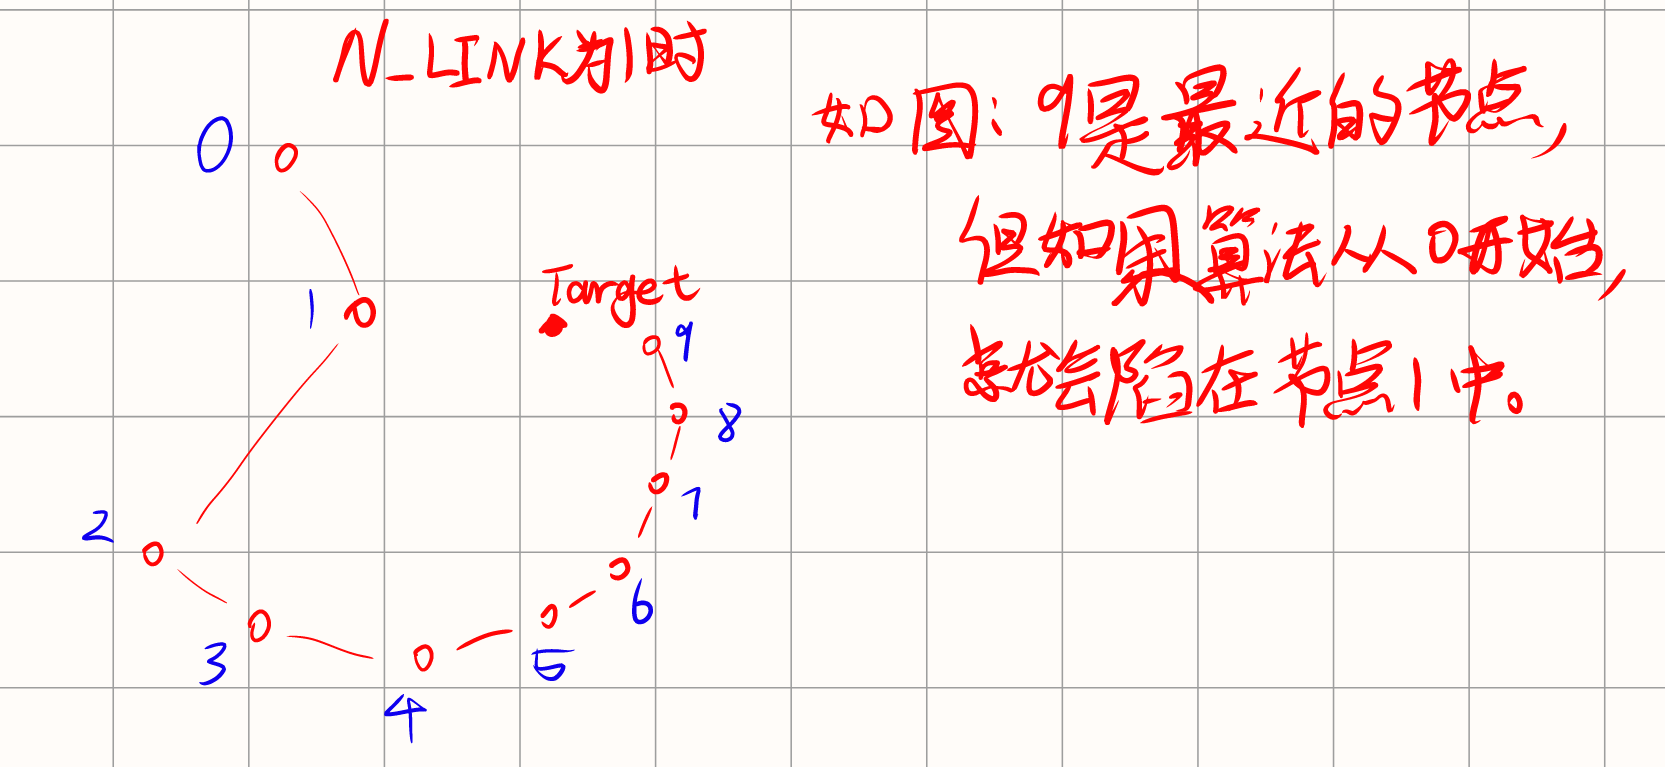
\includegraphics[width=0.6\textwidth]{img/local-minimun}
    \caption{Local Minimum}
\end{figure}

从图中也能看出,陷入局部最小值的一个显著影响因素就是 \texttt{N\_LINK} 参数,我在第一次提交时设置了 \texttt{N\_LINK}
为 2.
增加 \texttt{N\_LINK} 的值可以减小陷入局部最小值的可能性, 但是会导致每个节点和其他节点的连接变多,
会增大内存的占用和时间消耗.

\subsection{修改参数}

于是我斗胆一试,把 \texttt{N\_LINK} 逐渐增加,令我意外的是,结果不断变好,一路冲上 93 分,算法终于发挥了显著的速度优势.

\begin{figure}[H]
    \centering
    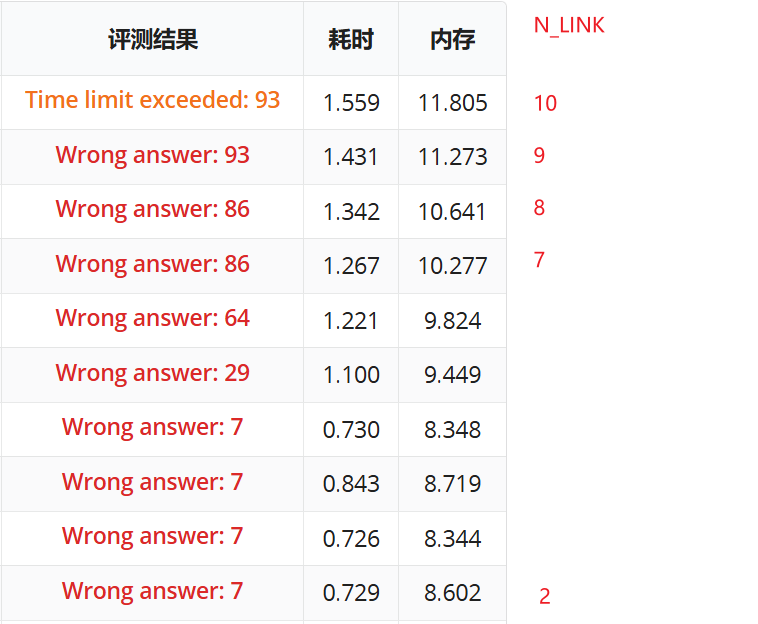
\includegraphics[width=0.8\textwidth]{img/hnsw-score-increasing}
    \caption{HNSW Score Increasing}
\end{figure}

\subsection{AC}

\texttt{1.559},很接近 1.5s 的时间限制,抱着撞撞运气的想法,以 \texttt{N\_LINK} 为 10 提交了几次,竟然真的给我撞出
AC 了 (代码中没有任何算法依靠随机生成).

\begin{figure}[H]
    \centering
    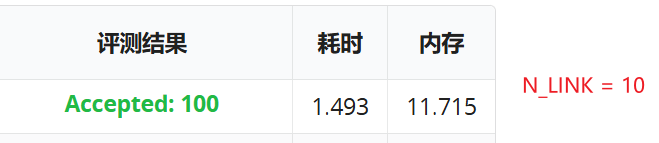
\includegraphics[width=0.6\textwidth]{img/ac}
    \caption{AC}
\end{figure}

\subsection{测试集时间性能分析}

在测试集 \texttt{b8000\_q45000\_k30\_d8\_1.in} 作为输入的情况下,时间性能分析如下:

\begin{verbatim}
Parameters: { DK_LAYER1: 100, DK_LAYER2: 500, DK_LAYER3: 1000, N_LINK: 10 }
Building Result { cnt: 8000, time(ms): 250, avg: 32000.000000 Hz }
Searching Result { cnt: 45000, time(ms) : 6032, avg: 7460.212202 Hz }
Total: 1350000, Correct: 1316681, Recall: 97.53%
\end{verbatim}

\begin{figure}[H]
    \centering
    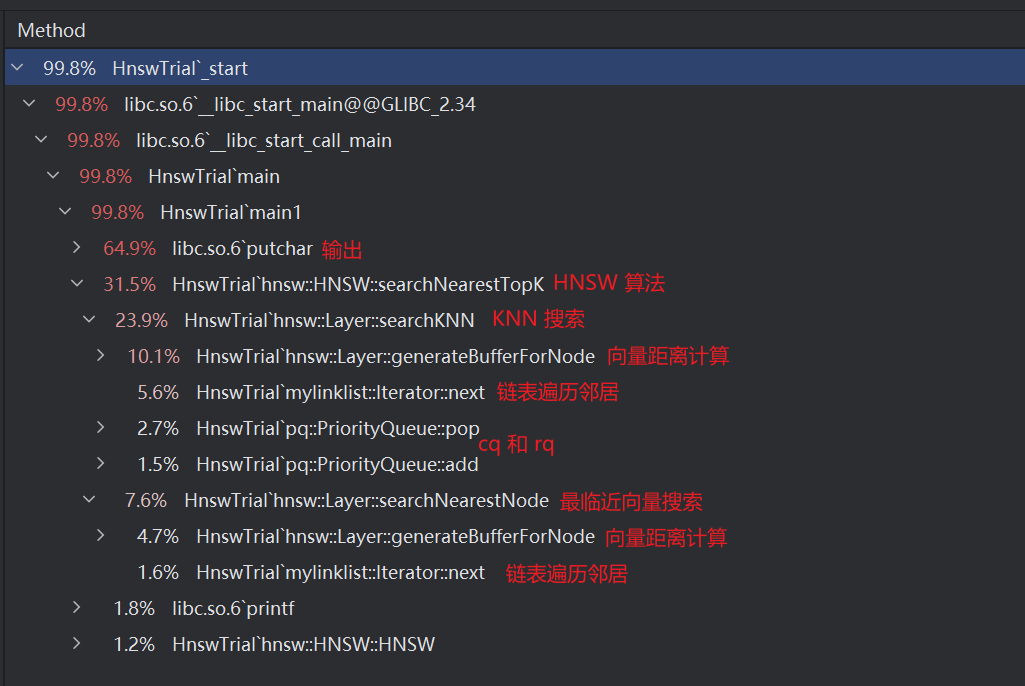
\includegraphics[width=0.8\textwidth]{img/hnsw-testdataset-profile}
    \caption{HNSW Test Dataset Profile}
\end{figure}

\subsection{中等数据集上的表现}

此算法在 \texttt{sift.in} 为输入时,表现如下:

\begin{verbatim}
Parameters: { DK_LAYER1: 100, DK_LAYER2: 500, DK_LAYER3: 1000, N_LINK: 10 }
Building Result { cnt: 1000000, time(ms): 471019, avg: 2123.056607 Hz }
Searching Result { cnt: 10000, time(ms) : 18920, avg: 528.541226 Hz }
Total: 1000000, Correct: 775206, Recall: 77.52%
\end{verbatim}